\documentclass[12pt, logo=tehranDLDL/ut]{tehranDLDL}
\usepackage{pgfplots}
\usepackage[american, siunitx]{circuitikz}
\usepackage{tikz-timing}

\suptitle{Experiment 1}
\supsubtitle{Sessions 1, 2, 3}
\title{Clock and Periodic Signal Generation}
\author{Katayoon Basharkhah \& Hadi Safari}
\preparer{\href{mailto:ktbasharkhah@gmail.com?subject=[DLDLab]\%20}{Katayoon Basharkhah}}
\supervisor{Professor Z. Navabi}
\university{University of Tehran}
\college{College of Engineering\\School of Electrical \& Computer Engineering}
\course[DLLab]{Digital Logic Laboratory}
\coursecode{ECE 045}
\courseurl{https://cecm.ut.ac.ir/course/view.php?id=2702}
\date{Spring 1398}

\graphicspath{{img/1/}}
\usetikzlibrary{positioning, shapes.multipart}

\begin{document}

\maketitle

\tableofcontents
\newpage

\section*{Introduction}
\addcontentsline{toc}{section}{Introduction}

The goal of this experiment is to introduce the concepts of static characteristics of digital logic gates, delay times, clock frequency generation and digital system using schematic diagram and \textit{Verilog} HDL.

By the end of this experiment, you should have learned:

\begin{itemize}
    \item Power supply, Function Generator, and Oscilloscope
    \item TTL 74 Series Basic Logic Gates 
    \item Different oscillator circuits (a LM555 timer IC, Schmitt trigger Oscillator)
    \item DE1 FPGA Educational Board
\end{itemize}

\section{Measure Static Characteristic of Inverter}
In this part, you will understand and measure the static characteristic of an inverter using 74LS04 TTL gate. The pin diagram of 74LS04 is shown in ~\fref{fig:74LS04}.

\begin{figure}[b]
    \centering
    \caption{74LS04 IC\label{fig:74LS04}}
    \resizebox{0.3\textwidth}{!}{
    \begin{circuitikz}
        % border
        \draw[very thick, fill={Black!10!White}] (0,0) -| (14,4) -| (0,2.75) -- (0,2.75) arc(90:-90:0.75) -- cycle;
        % NOTs
        \draw (2,1) node (nand21) [not port] {};
        \draw (1,0) |- (nand21.in);
        \draw (nand21.out) -| (3,0);
        \draw (6,1) node (nand61) [not port] {};
        \draw (5,0) |- (nand61.in);
        \draw (nand61.out) -| (7,0);
        \draw (10,1) node (nand101) [not port] {};
        \draw (9,0) |- (nand101.in);
        \draw (nand101.out) -| (11,0);
        \draw (4,3) node (nand43) [not port] {};
        \draw (3,4) |- (nand43.in);
        \draw (nand43.out) -| (5,4);
        \draw (4,3) node (nand43) [not port] {};
        \draw (3,4) |- (nand43.in);
        \draw (nand43.out) -| (5,4);
        \draw (8,3) node (nand83) [not port] {};
        \draw (7,4) |- (nand83.in);
        \draw (nand83.out) -| (9,4);
        \draw (12,3) node (nand123) [not port] {};
        \draw (11,4) |- (nand123.in);
        \draw (nand123.out) -| (13,4);
        % PINs
        \draw (0.5,0) rectangle (1.5,-1);
        \node at (1,-0.5) {\LARGE 1};
        \draw (2.5,0) rectangle (3.5,-1);
        \node at (3,-0.5) {\LARGE 2};
        \draw (4.5,0) rectangle (5.5,-1);
        \node at (5,-0.5) {\LARGE 3};
        \draw (6.5,0) rectangle (7.5,-1);
        \node at (7,-0.5) {\LARGE 4};
        \draw (8.5,0) rectangle (9.5,-1);
        \node at (9,-0.5) {\LARGE 5};
        \draw (10.5,0) rectangle (11.5,-1);
        \node at (11,-0.5) {\LARGE 6};
        \draw (12.5,0) rectangle (13.5,-1);
        \node at (13,-0.5) {\LARGE 7};
        \draw (0.5,4) rectangle (1.5,5);
        \node at (1,4.5) {\LARGE 14};
        \draw (2.5,4) rectangle (3.5,5);
        \node at (3,4.5) {\LARGE 13};
        \draw (4.5,4) rectangle (5.5,5);
        \node at (5,4.5) {\LARGE 12};
        \draw (6.5,4) rectangle (7.5,5);
        \node at (7,4.5) {\LARGE 11};
        \draw (8.5,4) rectangle (9.5,5);
        \node at (9,4.5) {\LARGE 10};
        \draw (10.5,4) rectangle (11.5,5);
        \node at (11,4.5) {\LARGE 9};
        \draw (12.5,4) rectangle (13.5,5);
        \node at (13,4.5) {\LARGE 8};
        % labels
        \node at (1,5.75) {\huge $V_\mathit{CC}$};
        \node at (13,-1.75) {\huge $\mathit{GND}$};
    \end{circuitikz}
    }
\end{figure}

\subsection{Voltage Transfer Characteristic}

The relationship between input and output of a logic gate is an important issue since the voltage level of a logic gate in a real world depends on the logic family resulting in values other than 1 and 0. The voltage transfer characteristic is a representation of output voltage variation when the input voltage changes continuously as in \fref{fig:vtc}.

\begin{figure}
    \centering
    \caption{Voltage transfer characteristic\label{fig:vtc}}
    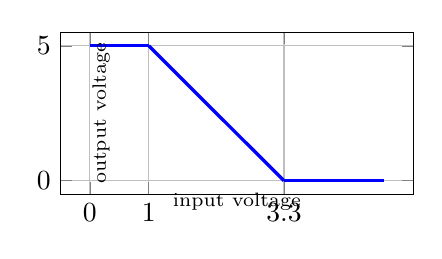
\begin{tikzpicture}
        \begin{axis}[grid=major, samples=10, smooth,
                xtick={0, 1, 3.3},xlabel={\scriptsize input voltage},
                ytick={0, 5},ylabel={\scriptsize output voltage},
                x label style={at={(axis cs:2.5,-0.1)},anchor=north},
                y label style={at={(axis cs:0.5,2.5)},anchor=south},
                scale=1,domain=0:5,height=0.3\textwidth, width=0.5\textwidth]
            \addplot[Blue, domain=0:1, very thick]
                plot (\x, 5);
            \addplot[Blue, domain=3.3:5, very thick]
                plot (\x, 0);
            \addplot[Blue, domain=1:3.3, very thick]
                plot (\x, {5 - 2.1739130435 * (\x - 1)});
       \end{axis}
    \end{tikzpicture}
\end{figure}

Construct the circuit shown in \fref{fig:vtc-setup}. The oscilloscope must be set in $X-Y$ mode in order to observe output variation based on the input. Hence, $\mathit{PIN}_1$ and $\mathit{PIN}_2$ are connected to $X$ and $Y$ channels, respectively. Adjust the function generator for a triangular input waveform which varies from \SI{0}{\volt} to \SI{+5}{\volt} when the input goes from \SI{0}{\volt} to \SI{+5}{\volt}, the output changes from $V_H$ to $V_L$ and then back. Report the $V_{O_H}$, $V_{O_L}$, $V_{I_L}$ and $V_{I_H}$ values in a table and answer these question in your report:
\begin{enumerate}
    \item Why are the values of $V_{O_H}$, $V_{O_L}$, $V_{I_L}$ and $V_{I_H}$ important?
    \item Find the nominal value of $V_{O_H}$, $V_{O_L}$ by referring to datasheet.
    \item Explain the hysteresis observed in VTC diagram.
\end{enumerate}

\begin{figure}
    \centering
    \caption{VTC determination set up\label{fig:vtc-setup}}
    \resizebox{0.7\textwidth}{!}{
    \begin{circuitikz}
        % border
        \draw[very thick, fill={Black!10!White}] (0,0) -| (14,4) -| (0,2.75) -- (0,2.75) arc(90:-90:0.75) -- cycle;
        \node[anchor=north, rotate=90] at (14, 2) {\huge 74LS04};
        % NOTs
        \draw (2,1) node (nand21) [not port] {};
        \draw (1,0) |- (nand21.in);
        \draw (nand21.out) -| (3,0);
        \draw (6,1) node (nand61) [not port] {};
        \draw (5,0) |- (nand61.in);
        \draw (nand61.out) -| (7,0);
        \draw (10,1) node (nand101) [not port] {};
        \draw (9,0) |- (nand101.in);
        \draw (nand101.out) -| (11,0);
        \draw (4,3) node (nand43) [not port] {};
        \draw (3,4) |- (nand43.in);
        \draw (nand43.out) -| (5,4);
        \draw (4,3) node (nand43) [not port] {};
        \draw (3,4) |- (nand43.in);
        \draw (nand43.out) -| (5,4);
        \draw (8,3) node (nand83) [not port] {};
        \draw (7,4) |- (nand83.in);
        \draw (nand83.out) -| (9,4);
        \draw (12,3) node (nand123) [not port] {};
        \draw (11,4) |- (nand123.in);
        \draw (nand123.out) -| (13,4);
        % PINs
        \draw (0.5,0) rectangle (1.5,-1);
        \node at (1,-0.5) {\LARGE 1};
        \draw (2.5,0) rectangle (3.5,-1);
        \node at (3,-0.5) {\LARGE 2};
        \draw (4.5,0) rectangle (5.5,-1);
        \node at (5,-0.5) {\LARGE 3};
        \draw (6.5,0) rectangle (7.5,-1);
        \node at (7,-0.5) {\LARGE 4};
        \draw (8.5,0) rectangle (9.5,-1);
        \node at (9,-0.5) {\LARGE 5};
        \draw (10.5,0) rectangle (11.5,-1);
        \node at (11,-0.5) {\LARGE 6};
        \draw (12.5,0) rectangle (13.5,-1);
        \node at (13,-0.5) {\LARGE 7};
        \draw (0.5,4) rectangle (1.5,5);
        \node at (1,4.5) {\LARGE 14};
        \draw (2.5,4) rectangle (3.5,5);
        \node at (3,4.5) {\LARGE 13};
        \draw (4.5,4) rectangle (5.5,5);
        \node at (5,4.5) {\LARGE 12};
        \draw (6.5,4) rectangle (7.5,5);
        \node at (7,4.5) {\LARGE 11};
        \draw (8.5,4) rectangle (9.5,5);
        \node at (9,4.5) {\LARGE 10};
        \draw (10.5,4) rectangle (11.5,5);
        \node at (11,4.5) {\LARGE 9};
        \draw (12.5,4) rectangle (13.5,5);
        \node at (13,4.5) {\LARGE 8};
        % func gen
        \draw[very thick, rounded corners] (-13,-3) rectangle (-6,0);
        \draw[rounded corners, fill=JungleGreen] (-12.5,-2.5) rectangle (-10.5,-0.5);
        \draw[thin, domain=-12.4:-10.6, samples=100, color=GreenYellow] plot(\x,{-1.5 + 0.9 * sin((600 * \x)});
        \node at (-9.5,0.5) {\huge Function Generator};
        \draw (-12.5,-3) rectangle (-11.5,-3.25);
        \draw (-7.5,-3) rectangle (-6.5,-3.25);
        \node[circle, fill] (func-gen) at (-8,-2.75) {};
        % oscope
        \draw[very thick, rounded corners] (-9,3) rectangle (-2,6);
        \draw[rounded corners, fill=JungleGreen] (-8.5,3.5) rectangle (-6.5,5.5);
        \draw[thin, domain=-8.4:-6.6, samples=100, color=GreenYellow] plot(\x,{4.5 + 0.9 * sin((600 * \x)});
        \node at (-5.5,6.5) {\huge Oscilloscope};
        \draw (-8.5,3) rectangle (-7.5,2.75);
        \draw (-3.5,3) rectangle (-2.5,2.75);
        \node[circle, fill, label={[above left, shift={(0.5,0)}]\Large ChI|X}] (oscope-x) at (-5,3.25) {};
        \node[circle, fill, label={[above right, shift={(-0.5,0)}]\Large ChII|Y}] (oscope-y) at (-4,3.25) {};
        % routing
        \draw (1,5) -- (1,5.5) node[vcc, scale=2] {};
        \draw (13,-1) -- (13,-1.5) node[ground, scale=2] {};
        \draw (func-gen) -- +(0, -1) -| (1,-1);
        \draw (oscope-x) |- (1,-2) -- (1,-1);
        \draw (oscope-y) |- (0.9,-1.5) arc(180:0:0.1) -- (1.1,-1.5) -- (3,-1.5) -- (3,-1);
    \end{circuitikz}
    }
\end{figure}

\section{Clock Generation}
In this part, you will understand different methods of clock generation in digital systems. 

\subsection{Ring Oscillator\label{sec:ring}}

One of the most important parameters in digital logic gates is the propagation delay, that is defined as the time from the 50\% point of input to the 50\% point of output, as shown in \fref{fig:timing}. There are also two more parameters named $t_{fall}$ and $t_{rise}$ that are measured as the time between 10\% and 90\% point of the signal and vice versa.

\begin{figure}
    \centering
    \caption{Timing diagram of a logic gate\label{fig:timing}}
    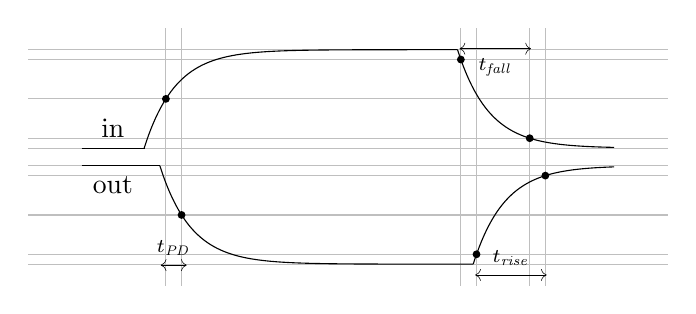
\begin{tikzpicture}
        \begin{axis}[grid=major, samples=100, smooth,ymajorticks=false,xmajorticks=false,axis line style={draw=none},
                xtick={0.6931471806, 1.1931471806, 10.1053605157, 10.6053605157, 12.302585093, 12.802585093},
                ytick={0.59, -0.59, 0.19, -0.19, 0.99, -0.99, 0.09, -0.09, 1.09, -1.09},
                scale=1,domain=-2:15,height=0.4\textwidth, width=0.8\textwidth]
            % in
            \addplot[domain=-2:0]
                plot (\x, 0.09 + 0);
            \addplot[domain=0:10]
                plot (\x, { 0.09 + 1 - exp(0-\x) });
            \addplot[domain=10:15]
                plot (\x, { 0.09 + exp(10-\x) });
            % out
            \addplot[domain=-2:0.5]
                plot (\x, -0.09 + 0);
            \addplot[domain=0.5:10.5]
                plot (\x, { -0.09 - (1 - exp(0.5-\x)) });
            \addplot[domain=10.5:15]
                plot (\x, { -0.09 - exp(10.5-\x) });
            % markers
            \node[circle,fill,inner sep=1pt] at (axis cs:0.6931471806,0.59) {};
            \node[circle,fill,inner sep=1pt] at (axis cs:1.1931471806,-0.59) {};
            \node[circle,fill,inner sep=1pt] at (axis cs:10.1053605157,0.99) {};
            \node[circle,fill,inner sep=1pt] at (axis cs:10.6053605157,-0.99) {};
            \node[circle,fill,inner sep=1pt] at (axis cs:12.302585093,0.19) {};
            \node[circle,fill,inner sep=1pt] at (axis cs:12.802585093,-0.19) {};
            % labels
            \node[anchor=south] at (axis cs:-1,0.1) {in};
            \node[anchor=north] at (axis cs:-1,-0.1) {out};
            \node (in_mid) at (axis cs:0.6931471806,-1.1) {};
            \node (out_mid) at (axis cs:1.1931471806,-1.1) {};
            \node (in_beg) at (axis cs:10.1053605157,1.1) {};
            \node (out_beg) at (axis cs:10.6053605157,-1.2) {};
            \node (in_end) at (axis cs:12.302585093,1.1) {};
            \node (out_end) at (axis cs:12.802585093,-1.2) {};
            \draw[<->,shorten >= -4pt,shorten <= -4pt, very thin] (in_mid) -- (out_mid) node[midway, above] {\scriptsize$t_\mathit{PD}$};
            \draw[<->,shorten >= -4pt,shorten <= -4pt, very thin] (in_beg) -- (in_end) node[midway, below] {\scriptsize$t_\mathit{fall}$};
            \draw[<->,shorten >= -4pt,shorten <= -4pt, very thin] (out_beg) -- (out_end) node[midway, above] {\scriptsize$t_\mathit{rise}$};
       \end{axis}
    \end{tikzpicture}
\end{figure}

The delay of logic gates is very small and this imposes a large bandwidth. So, measuring this delay directly using a relatively low-cost oscilloscope may be difficult. An alternative method for measuring this parameter is using a \textit{ring oscillator} as shown in \fref{fig:ring}. A ring oscillator is composed of a chain of odd number of inverters, in which output of last inverter is connected to the input of first one. The time at which a value feeds back to the same node is the time period of the ring oscillator which equals $2N*Delay_{inv}$, where $N$ is the odd number and $Delay_{inv}$ is the delay of each inverter gate. The delay of each single inverter can be determined by measuring the total delay.

\begin{figure}
    \centering
    \caption{Ring oscillator\label{fig:ring}}
    \resizebox{0.3\textwidth}{!}{
    \begin{circuitikz}
        \draw
            (1,0) node (nand1) [not port] {}
            (3,0) node (nand2) [not port] {}
            (5,0) node (nand3) [not port] {}
        ;
        \draw (nand1.out) -- (nand2.in);
        \draw (nand2.out) -- (nand3.in);
        \draw (nand3.out) -- (6,0) -- (6,1) -- (0,1) -- (0,0) -- (nand1.in);
    \end{circuitikz}
    }
\end{figure}

Construct the circuit shown in \fref{fig:ring_74LS04} with as little wire as possible. You should wire up three of six inverters to a chain.

\begin{enumerate}
    \item Measure the propagation delay of the chain by measuring the period time of the output.
    \item Measure the delay of a single inverter and compare it with the delay in 7404 TTL specification. You can also use a 74HC14 IC for this part.
\end{enumerate}

\begin{figure}
    \centering
    \caption{Ring oscillator using 74LS04\label{fig:ring_74LS04}}
    \resizebox{0.4\textwidth}{!}{
    \begin{circuitikz}
        % border
        \draw[very thick, fill={Black!10!White}] (0,0) -| (14,4) -| (0,2.75) -- (0,2.75) arc(90:-90:0.75) -- cycle;
        \node[anchor=north, rotate=90] at (14, 2) {\huge 74LS04};
        % NOTs
        \draw (2,1) node (nand21) [not port,color=Maroon] {};
        \draw[Maroon] (1,0) |- (nand21.in);
        \draw[Maroon] (nand21.out) -| (3,0);
        \draw (6,1) node (nand61) [not port,color=Maroon] {};
        \draw[Maroon] (5,0) |- (nand61.in);
        \draw[Maroon] (nand61.out) -| (7,0);
        \draw (10,1) node (nand101) [not port,color=Maroon] {};
        \draw[Maroon] (9,0) |- (nand101.in);
        \draw[Maroon] (nand101.out) -| (11,0);
        \draw (4,3) node (nand43) [not port] {};
        \draw (3,4) |- (nand43.in);
        \draw (nand43.out) -| (5,4);
        \draw (4,3) node (nand43) [not port] {};
        \draw (3,4) |- (nand43.in);
        \draw (nand43.out) -| (5,4);
        \draw (8,3) node (nand83) [not port] {};
        \draw (7,4) |- (nand83.in);
        \draw (nand83.out) -| (9,4);
        \draw (12,3) node (nand123) [not port] {};
        \draw (11,4) |- (nand123.in);
        \draw (nand123.out) -| (13,4);
        % PINs
        \draw (0.5,0) rectangle (1.5,-1);
        \node at (1,-0.5) {\LARGE 1};
        \draw (2.5,0) rectangle (3.5,-1);
        \node at (3,-0.5) {\LARGE 2};
        \draw (4.5,0) rectangle (5.5,-1);
        \node at (5,-0.5) {\LARGE 3};
        \draw (6.5,0) rectangle (7.5,-1);
        \node at (7,-0.5) {\LARGE 4};
        \draw (8.5,0) rectangle (9.5,-1);
        \node at (9,-0.5) {\LARGE 5};
        \draw (10.5,0) rectangle (11.5,-1);
        \node at (11,-0.5) {\LARGE 6};
        \draw (12.5,0) rectangle (13.5,-1);
        \node at (13,-0.5) {\LARGE 7};
        \draw (0.5,4) rectangle (1.5,5);
        \node at (1,4.5) {\LARGE 14};
        \draw (2.5,4) rectangle (3.5,5);
        \node at (3,4.5) {\LARGE 13};
        \draw (4.5,4) rectangle (5.5,5);
        \node at (5,4.5) {\LARGE 12};
        \draw (6.5,4) rectangle (7.5,5);
        \node at (7,4.5) {\LARGE 11};
        \draw (8.5,4) rectangle (9.5,5);
        \node at (9,4.5) {\LARGE 10};
        \draw (10.5,4) rectangle (11.5,5);
        \node at (11,4.5) {\LARGE 9};
        \draw (12.5,4) rectangle (13.5,5);
        \node at (13,4.5) {\LARGE 8};
        % routing
        \draw (1,5) -- (1,5.5) node[vcc, scale=2] {\SI{5}{\volt}};
        \draw (13,-1) -- (13,-1.5) node[ground, scale=2] {};
        \draw[Maroon] (3,-1) -- (3,-1.5) -| (5,-1);
        \draw[Maroon] (7,-1) -- (7,-1.5) -| (9,-1);
        \draw[Maroon] (1,-1) -- (1,-2) -| (11,-1);
        \draw (1,-2) -- (0,-2) node[circ, label={[below]\huge output}] {};
    \end{circuitikz}
    }
\end{figure}

\designverification{}

\subsection{LM555 timer}

LM555 is among the devices can be used for generating clock signal or time delays. The pin layout of this IC can be seen in \fref{fig:LM555}. 

\begin{figure}
    \centering
    \caption{LM555 timer pin-out\label{fig:LM555}}
    \resizebox{0.5\textwidth}{!}{
    \begin{circuitikz}
        % border
        \draw[very thick, fill={Black!10!White}] (0,8) |- (4,0) |- (2.5,8) -- (2.5,8) arc(0:-180:0.5) -- cycle;
        % inside
        \draw (1.5,2.5) rectangle (2.5,3.5);
        \node at (2,3) {F/F};
        \node[pnp,yscale=-1] (rst_trans) at (1,1) {};
        \draw (rst_trans.E) -- +(1,0) node[ocirc, label={[right]$V_\mathit{REF}$}] {};
        \draw (rst_trans.C) -| (1.75,2.5);
        \node[buffer, scale=-0.5, label={[above, text width=1.5cm]\scriptsize output stage}] (out_buf) at (1,3) {};
        \node[op amp, scale=-0.5] (ctrl_opamp) at (3.25, 2.75) {};
        \node at (3.25, 2.75) {\footnotesize cmp};
        \draw (ctrl_opamp.out) -- (2.5,2.75);
        \draw (out_buf.in) --(1.5,3);
        \node[op amp, xscale=0.5, yscale=-0.5] (trigger_opamp) at (1, 5.25) {};
        \node at (1, 5.25) {\footnotesize cmp};
        \node[npn,rotate=90, yscale=-1, label={[text width=1.5cm]\scriptsize discharging transistor}] (dis_trans) at (3,5) {};
        \draw (dis_trans.B) |- (2.5,3.25);
        \draw (dis_trans.E) -- +(-0,0) node[ground] {};
        \draw (trigger_opamp.out) -| (1.75,3.5);
        \node[resistorshape, scale=0.5, label={\footnotesize R}] (r_left) at (1,7) {};
        \node[resistorshape, scale=0.5, label={\footnotesize R}] (r_mid) at (2,7) {};
        \node[resistorshape, scale=0.5, label={\footnotesize R}] (r_right) at (3,7) {};
        \draw (0,7) -- (r_left.left);
        \draw (r_left.right) -- (r_mid.left);
        \draw (r_mid.right) -- (r_right.left);
        \draw (r_right.right) -- (4,7);
        \draw (1.5,7) -- +(0,-0.5) -| (trigger_opamp.+);
        \draw (trigger_opamp.-) -- (0,5);
        \draw (out_buf.out) -- (0,3);
        \draw (ctrl_opamp.+) -- (4,3);
        \draw (ctrl_opamp.-) |- (4,1);
        \draw (rst_trans.B) -- (0,1);
        \draw (dis_trans.C) -- (4,5);
        \draw (r_right.left) +(-0.1,0) |- (4,1);
        % PINs
        \draw (0,0.5) rectangle (-1,1.5);
        \node at (-0.5,1) {4};
        \node at (-2.5,1) {\ol{reset}};
        \draw (0,2.5) rectangle (-1,3.5);
        \node at (-0.5,3) {3};
        \node at (-2.5,3) {output};
        \draw (0,4.5) rectangle (-1,5.5);
        \node at (-0.5,5) {2};
        \node at (-2.5,5) {\ol{trigger}};
        \draw (0,6.5) rectangle (-1,7.5);
        \node at (-0.5,7) {1};
        \node at (-2.5,7) {$\textit{GND}$};
        \draw (4,0.5) rectangle (5,1.5);
        \node at (4.5,1) {5};
        \node at (6.5,1) {control voltage};
        \draw (4,2.5) rectangle (5,3.5);
        \node at (4.5,3) {6};
        \node at (6.5,3) {threshold};
        \draw (4,4.5) rectangle (5,5.5);
        \node at (4.5,5) {7};
        \node at (6.5,5) {discharge};
        \draw (4,6.5) rectangle (5,7.5);
        \node at (4.5,7) {8};
        \node at (6.5,7) {$V_\textit{CC}$};
    \end{circuitikz}
    }
\end{figure}

This IC operates in three modes: Monostable, Bistable and Astable. The astable mode that we use in this experiment allows the timer to operate as an oscillator that outputs a continuous rectangular pulse of a required frequency. For astable operation, we need two resistors and one capacitor to design a circuit that operates at the frequency required. The timing during which the output is either high or low is determined by these externally connected resistors and capacitors. Note that the durations of the low and high states may be different. \Fref{fig:LM555_astable} illustrates an LM555 configuration for astable mode operation.

\begin{figure}
    \centering
    \caption{LM555 in astable mode\label{fig:LM555_astable}}
    \resizebox{0.5\textwidth}{!}{
    \begin{circuitikz}
        % border
        \draw[very thick, fill={Black!10!White}] (0,8) |- (4,0) |- (2.5,8) -- (2.5,8) arc(0:-180:0.5) -- cycle;
        \node at (2,-0.5) {\LARGE LM555};
        % PINs
        \draw (0,0.5) rectangle (-1,1.5);
        \node at (-0.5,1) {4};
        \node at (1,1) {\Large \ol{RST}};
        \draw (0,2.5) rectangle (-1,3.5);
        \node at (-0.5,3) {3};
        \node at (1,3) {\Large OUT};
        \draw (0,4.5) rectangle (-1,5.5);
        \node at (-0.5,5) {2};
        \node at (1,5) {\Large \ol{TRIG}};
        \draw (0,6.5) rectangle (-1,7.5);
        \node at (-0.5,7) {1};
        \node at (1,7) {\Large $\textit{GND}$};
        \draw (4,0.5) rectangle (5,1.5);
        \node at (4.5,1) {5};
        \node at (3,1) {\Large CONT};
        \draw (4,2.5) rectangle (5,3.5);
        \node at (4.5,3) {6};
        \node at (3,3) {\Large THRES};
        \draw (4,4.5) rectangle (5,5.5);
        \node at (4.5,5) {7};
        \node at (3,5) {\Large DISCH};
        \draw (4,6.5) rectangle (5,7.5);
        \node at (4.5,7) {8};
        \node at (3,7) {\Large $V_\textit{CC}$};
        % wiring
        \node[polarcapacitorshape, rotate=90, scale=2, label={[left]\Large\SI{10}{\nano\farad}}] (cap_left) at (6, -2) {};
        \node[polarcapacitorshape, rotate=90, scale=2, label={[right, label distance=-5em]\Large\SI{10}{\nano\farad}}] (cap_right) at (9, -2) {};
        \node[resistorshape, rotate=90, scale=2, label={[right, label distance=-5em]\Large$R_1$}] (res_top) at (9, 7) {};
        \node[resistorshape, rotate=90, scale=2, label={[right, label distance=-5em]\Large$R_2$}] (res_bottom) at (9, 3) {};
        \draw[very thick] (-1,7) -| (-4,-3) node[ground, scale=2] (gnd) {\scriptsize$\mathit{GND}$};
        \draw[very thick] (5,1) -| (cap_left.right);
        \draw[very thick] (cap_left.left) |- (gnd);
        \draw[very thick] (cap_right.left) |- (gnd);
        \draw[Red,very thick] (res_top.right) |- (-4,9) node[vcc, scale=2, color=Red] (vcc) {\scriptsize$V_\mathit{CC}$};
        \draw[Red,very thick] (5,7) -- +(1,0) |- (vcc);
        \draw[Red,very thick] (-1,1) -- +(-1,0) |- (vcc);
        \draw[NavyBlue,very thick] (res_top.left) -- (res_bottom.right);
        \draw[NavyBlue,very thick] (res_bottom.left) -- (cap_right.right);
        \draw[NavyBlue,very thick] (5,5) -- (9,5);
        \draw[NavyBlue,very thick] (5,3) -| (7.5,-1);
        \draw[NavyBlue,very thick] (-1,5) -- +(-2,0) |- (9,-1);
        \draw[Green,very thick] (-1,3) -- (-6,3) node[circ, scale=2] {\scriptsize output};
    \end{circuitikz}
    }
\end{figure}

The external capacitor $C$ charges through $R_1 + R_2$ and discharges through $R_2$. Thus, the duty cycle and frequency may be precisely set by selecting the right combination of resistances and capacitance. According to \fref{fig:LM555} and \fref{fig:LM555_astable}, the charge time (output high) is given by $T_1 =0.693 * (R_1+ R_2) * C$ and the discharge time (output low) by $T_2 = 0.693 * R_2 * C$. Thus, the total time period of square wave is $T = T_1 + T_2 = 0.693 * (R_1 +2R_2) * C$. Consequently, the frequency of oscillation is $\frac{1}{T}$. The duty cycle also can be computed by $\frac{R_1 + R_2}{R_1 + 2 R_2}$.

These equations describe how we can choose these three values to decide on the frequency and the high and low durations of our signal. With the LM555 timer, the default value of $R_1$ in this configuration is \SI{1}{\kilo\ohm} and this means that we cannot get a perfect 50\% duty cycle. (If we make $R_2 \gg R_1$ then we can get close.)

Do the following work. Your report must include the procedure you followed, as well as any observation and results.

\begin{enumerate}
    \item Implement the LM555 in astable mode using the wiring diagram from \fref{fig:LM555_astable} and observe the output on oscilloscope. Measure the clock frequency and the duty cycle.
    \item Change the value of $R_2$ resistors to produce different clock frequencies. To do so, $R_2$ should be \SIlist{1; 10; 100}{\kilo\ohm}. Calculate the frequency and duty cycle using above equations and compare them to the clock signal you see on the oscilloscope.
\end{enumerate}

\designverification{}

\subsection{Schmitt Trigger Oscillator}

Below you can see the realization of the Schmitt inverter oscillator.

\begin{figure}[b]
    \centering
    \caption{Schmitt inverter oscillator circuit\label{fig:schmitt}}
    \resizebox{0.3\textwidth}{!}{
        \begin{circuitikz}
            \node (invsch) [invschmitt,label={[below right]{\quad74LS14}}] at (2,2) {};
            \draw
                (5,0) node[ocirc] {} -- (0,0) to[C] (0,2) -- (0,4)
                to[R] (4,4) -- (4,2) -- (5,2) node[ocirc] {}
                (0,2) -- (invsch.in)
                (invsch.out) -- (4,2)
                (invsch) ++(0,-0.25) -- ++(0, -0.5) node[ground] {}
                (invsch) ++(0,0.25) -- ++(0, 0.5) node[vcc,label={[above right]\quad\SI{5}{\volt}}] {}
            ;
        \end{circuitikz}
    }

\end{figure}

In the the Schmitt inverter oscillator, $f = \frac{\alpha}{RC}$, where $\alpha$ is a constant.

\begin{enumerate}
    \item Considering the given equation, try the circuit with different values for the resistor and
the capacitor and observe the changes. Use \SIlist{470; 1e3; 2e3}{\ohm} for $R_1$ and \SI{10}{\nano\farad} for $C$.
    \item Find $\alpha$ parameter.
\end{enumerate}

\designverification{}

\subsection{Synchronous Counter as a Frequency Divider\label{sec:counter}}

Different clock signals can be produced by the aforementioned methods, but not all of them are suitable for all applications. Consider a \SI{1}{\hertz} clock signal which can be easily produced by a LM555 timer. The timing error of this signal can be 1-2\%, which is too much for a low frequency like this, while this error range is acceptable for higher frequencies. So, a higher frequency can be chosen and then a frequency divider can reduce the frequency to the desired one.

Counters can be used as a frequency divider. 74LS191 is a synchronous 4-bit up/down counter. As \fref{fig:74LS191} shows, it has 4 inputs $A$-$D$, 4 outputs $Q_A$-$Q_D$ and a parallel load, which allows for presetting an initial value for the counter. With this pin layout two counters can be cascaded when the modulus is more than 4 bits.

\begin{figure}
    \centering
    \caption{Pin layout of 74LS191\label{fig:74LS191}}
    \resizebox{0.4\textwidth}{!}{
    \begin{circuitikz}
        % border
        \draw[very thick, fill={Black!10!White}] (0,16) |- (7,0) |- (5,16) -- (4.5,16) arc(0:-180:1) -- cycle;
        \node at (3.5,0.5) {\LARGE 74LS191};
        % PINs
        \draw (0,0.25) rectangle (-1.5,1.75);
        \node at (-0.75,1) {\Large 8};
        \node at (-3,1) {\Large $\mathit{GND}$};
        \draw (0,2.25) rectangle (-1.5,3.75);
        \node at (-0.75,3) {\Large 7};
        \node at (-3,3) {\Large $Q_D$ (output)};
        \draw (0,4.25) rectangle (-1.5,5.75);
        \node at (-0.75,5) {\Large 6};
        \node at (-3,5) {\Large $Q_C$ (output)};
        \draw (0,6.25) rectangle (-1.5,7.75);
        \node at (-0.75,7) {\Large 5};
        \node at (-3,7) {\Large down/\ol{up}};
        \draw (0,8.25) rectangle (-1.5,9.75);
        \node at (-0.75,9) {\Large 4};
        \node at (-3,9) {\Large \ol{$G$ (enable)}};
        \draw (0,10.25) rectangle (-1.5,11.75);
        \node at (-0.75,11) {\Large 3};
        \node at (-3,11) {\Large $Q_A$ (output)};
        \draw (0,12.25) rectangle (-1.5,13.75);
        \node at (-0.75,13) {\Large 2};
        \node at (-3,13) {\Large $Q_B$ (output)};
        \draw (0,14.25) rectangle (-1.5,15.75);
        \node at (-0.75,15) {\Large 1};
        \node at (-3,15) {\Large $B$ (input)};
        \draw (7,0.25) rectangle (8.5,1.75);
        \node at (7.75,1) {\Large 9};
        \node at (10,1) {\Large $D$ (input)};
        \draw (7,2.25) rectangle (8.5,3.75);
        \node at (7.75,3) {\Large 10};
        \node at (10,3) {\Large $C$ (input)};
        \draw (7,4.25) rectangle (8.5,5.75);
        \node at (7.75,5) {\Large 11};
        \node at (10,5) {\Large \ol{load}};
        \draw (7,6.25) rectangle (8.5,7.75);
        \node at (7.75,7) {\Large 12};
        \node[text width=7em] at (10,7) {\Large max/\ol{min} output};
        \draw (7,8.25) rectangle (8.5,9.75);
        \node at (7.75,9) {\Large 13};
        \node[text width=7em] at (10,9) {\Large \ol{ripple clock output}};
        \draw (7,10.25) rectangle (8.5,11.75);
        \node at (7.75,11) {\Large 14};
        \node at (10,11) {\Large clock};
        \draw (7,12.25) rectangle (8.5,13.75);
        \node at (7.75,13) {\Large 15};
        \node at (10,13) {\Large $A$ (input)};
        \draw (7,14.25) rectangle (8.5,15.75);
        \node at (7.75,15) {\Large 16};
        \node at (10,15) {\Large $V_\mathit{CC}$};
    \end{circuitikz}
    }
\end{figure}

The timing diagram of 74LS191 is shown in \fref{fig:74LS191_timing}. When up counting is desired the initial value is obtained by:
$$\mathit{Initial\ value} = \mathit{Maximum\ value} - \mathit{Modulus}$$

\begin{figure}
    \centering
    \caption{Timing diagram of 74LS191\label{fig:74LS191_timing}}
    % \resizebox{0.6\textwidth}{!}{
    \begin{tikztimingtable}
        \ol{load}         & 2H N(Lst) 1.5L N(Let) 24.5H \\
        $A$               & 1L 3H 24U \\
        $B$               & 1L 3L 24U \\
        $C$               & 1L 3H 24U \\
        $D$               & 1L 3H 24U \\
        $DCBA$            & 1D{0} 3D{13} 24U \\
        down/\ol{up}      & 1H 13.5L 13.5H \\
        \ol{enable}       & 1H 11.5L N(Ist) 4HN (Iet) 11.5L \\
        clock             & [C] 4{C} N(Ust) 14{C} N(Dst) 10{C} \\
        $Q_A$             & UU HH LL HH LL HH LL LL LL HH LL HH LL HH \\
        $Q_B$             & UU LL HH HH LL LL HH HH HH LL LL HH HH LL \\
        $Q_C$             & UU HH HH HH LL LL LL LL LL LL LL HH HH HH \\
        $Q_D$             & UU HH HH HH LL LL LL LL LL LL LL HH HH HH \\
        $Q_DQ_CQ_BQ_A$    & UU 2D{13} 2D{14} 2D{15} 2D{0} 2D{1} 2D{2} 2D{2} 2D{2} 2D{1} 2D{0} 2D{15} 2D{14} 2D{13} \\
        max/\ol{min}      & UU LL LL HH LL LL LL LL LL LL HH LL LL LL \\
        \ol{ripple clock} & UU HH HH HL HH HH HH HH HH HH HL HH HH HH \\
        & 2S N(Ls) 1.5S N(Le) 0.5S N(Us) 8.5S N(Ue) N(Is) 4S N(Ie) 1.5S N(Ds) 10S N(De) \\
        \extracode
        \draw[<->] (Ls) -- (Le) node[midway, below] {load};
        \draw[<->] (Us) -- (Ue) node[midway, below] {count up};
        \draw[<->] (Is) -- (Ie) node[midway, below] {inhibit};
        \draw[<->] (Ds) -- (De) node[midway, below] {count down};
        \draw[help lines] (Ls) -- (Lst);
        \draw[help lines] (Le) -- (Let);
        \draw[help lines] (Is) -- (Ist);
        \draw[help lines] (Ie) -- (Iet);
        \draw[help lines] (Us) -- (Ust);
        \draw[help lines] (Ds) -- (Dst);
    \end{tikztimingtable}
    % }
\end{figure}

Construct a divide by 113 synchronous counter as shown in \fref{fig:74LS193_freq_divider}. You should:
\begin{enumerate}
    \item Use the ring oscillator to generate a \SI{20}{\mega\hertz} clock signal.
    \item Connect the generated clock to the count up pin of counter.
    \item Preset the counter at the initial value.
    \item Record the results of carry out of the MSB counter and measure its frequency, compare the results with the input.
\end{enumerate}

\begin{figure}
    \centering
    \caption{Frequency divider using 74LS193\label{fig:74LS193_freq_divider}}
    \resizebox{0.9\textwidth}{!}{
    \begin{circuitikz}
        % left
        \draw[thick, fill={Black!10!White}] (0,0) rectangle (7,3);
        \node at (3.5,2) {\Large 74LS191};
        \node at (3.5,1) {\Large LSB};
        \draw (1,3) -- ++(0,1) node[vcc] {};
        \draw (1,0) -- ++(0,-1) node[ground] {};
        \node[ocirc,scale=2] (lsb-ld) at (2,3) {};
        \draw (3,3) -- ++(0,1) node[circ] {} +(0,0.3) node {1};
        \draw (4,3) -- ++(0,1) node[circ] {} +(0,0.3) node {1};
        \draw (5,3) -- ++(0,1) node[circ] {} +(0,0.3) node {1};
        \draw (6,3) -- ++(0,1) node[circ] {} +(0,0.3) node {1};
        \draw (3,0) -- ++(0,-1) node[circ] {};
        \draw (4,0) -- ++(0,-1) node[circ] {};
        \draw (5,0) -- ++(0,-1) node[circ] {};
        \draw (6,0) -- ++(0,-1) node[circ] {};
        \node[ocirc,scale=2] (lsb-rclk) at (7,1) {};
        \node at (6,1) {ripple clock};
        \node at (6,2) {max/min};
        \node at (0.5,2) {clock};
        \node at (2,2.75) {load};
        \node at (3,2.75) {$A$};
        \node at (4,2.75) {$B$};
        \node at (5,2.75) {$C$};
        \node at (6,2.75) {$D$};
        \node at (3,0.25) {$Q_A$};
        \node at (4,0.25) {$Q_B$};
        \node at (5,0.25) {$Q_C$};
        \node at (6,0.25) {$Q_D$};
        % right
        \draw[thick, fill={Black!10!White}] (9,0) rectangle (16,3);
        \node at (12.5,2) {\Large 74LS191};
        \node at (12.5,1) {\Large MSB};
        \draw (9+1,3) -- ++(0,1) node[vcc] {};
        \draw (9+1,0) -- ++(0,-1) node[ground] {};
        \node[ocirc,scale=2] (msb-ld) at (9+2,3) {};
        \draw (9+3,3) -- ++(0,1) node[circ] {} +(0,0.3) node {0};
        \draw (9+4,3) -- ++(0,1) node[circ] {} +(0,0.3) node {0};
        \draw (9+5,3) -- ++(0,1) node[circ] {} +(0,0.3) node {0};
        \draw (9+6,3) -- ++(0,1) node[circ] {} +(0,0.3) node {1};
        \draw (9+3,0) -- ++(0,-1) node[circ] {};
        \draw (9+4,0) -- ++(0,-1) node[circ] {};
        \draw (9+5,0) -- ++(0,-1) node[circ] {};
        \draw (9+6,0) -- ++(0,-1) node[circ] {};
        \node[ocirc,scale=2] (msb-rclk) at (9+7,1) {};
        \node at (9+6,1) {ripple clock};
        \node at (9+6,2) {max/min};
        \node at (9+0.5,2) {clock};
        \node at (9+2,2.75) {load};
        \node at (9+3,2.75) {$A$};
        \node at (9+4,2.75) {$B$};
        \node at (9+5,2.75) {$C$};
        \node at (9+6,2.75) {$D$};
        \node at (9+3,0.25) {$Q_A$};
        \node at (9+4,0.25) {$Q_B$};
        \node at (9+5,0.25) {$Q_C$};
        \node at (9+6,0.25) {$Q_D$};
        % wiring
        \draw (7,2) -- (9,2);
        \draw (msb-rclk) -| ++(1,3.75) -| (msb-ld);
        \draw (msb-rclk) -| ++(1,3.75) -| (lsb-ld);
        \node[vsourcesquareshape, scale=1.5, label={clock oscillator}] (src) at (-2,2) {};
        \draw (src.right) -- (0,2);
    \end{circuitikz}
    }
\end{figure}

\designverification{}

\section{FPGA Design}

In this part, you will be familiar with FPGA design. You will learn how to run and program a Verilog code on a FPGA board. The FPGA board that you will use in this and all other experiments until the end of the semester is \textit{Altera DE1} board. \Fref{fig:de1} shows the layout of the board and indicates the location of the connectors and key components.

\begin{figure}
    \centering
    \caption{Altera DE1 board\label{fig:de1}}
    \includegraphics[width=\textwidth]{de1.png}
\end{figure}

In this part you should use a FPGA to observe and calculate the frequency of a ring oscillator. You will use the circuits of previous sections along with FPGA as shown in \fref{fig:74LS74}. There are many parts which should be considered in designing such system. Below is a short description of these parts and what you should follow for this experiment.

\subsection{Ring Oscillator}

Use the ring oscillator of \fref{sec:ring} for this part. Use 3 of 6 inverters of 74LS14 IC to generate a \SI{20}{\mega\hertz} clock frequency. You can also use other types of inverters, like 74LS04, to produce a high frequency clock. Pay attention to the fact  that the inverter delays are different. See the datasheet of each inverter.

\subsection{Counter}

Use the counter of \fref{sec:counter}. Design a divide-by-50 counter. Connect the output of ring oscillator to the input of counter and observe the results. Check the output frequency of the counter if it is correctly divided by 50. It should be \SI{400}{\kilo\hertz}.

\subsection{Voltage Level Converter}

When the term logical 0 (GND) is used, it means almost \SI{0}{\volt} voltage, but logical 1 can mean different values for the $V_\mathit{CC}$ voltage (e.g. \SIlist{5; 3.3; 2.8}{\volt}). If all devices used in the circuit have the same voltage as logical 1 it would work correctly, but sometimes there are devices in the same circuit which expect different $V_\mathit{CC}$s. In such situations, \textit{level shifter}s are used. Level shifter has two sides: one dedicated to the high voltage $V_\mathit{CC}$ (HV) and one side to low voltage $V_\mathit{CC}$ (LV). In \textit{level converter} both sides have $\mathit{GND}$ and $V_\mathit{CC}$ pins; $\mathit{GND}$s are connected to the shared ground, HV to the higher $V_\mathit{CC}$, and LV to the lower $V_\mathit{CC}$. There are also four I/O pins on the HV side, and four on the LV side. Any of this pins can be driven by logical 1s and 0s, and the corresponding pin would change. For example, in the circuit shown in \fref{fig:level_conv}, FPGA uses \SI{3.3}{\volt} as $V_\mathit{CC}$ and ICs have \SI{5}{\volt} $V_\mathit{CC}$s, if HV1 is driven by \SI{5}{\volt}, LV1 would have the value \SI{3.3}{\volt}, and if $LV_2$ is driven by \SI{3.3}{\volt}, you can see \SI{5}{\volt} on $HV_2$ pin, and \SI{0}{\volt} on any pin would result \SI{0}{\volt} on the corresponding pin.

It is obvious that connected pins cannot be driven together, for example if $HV_4$ is driven, FPGA cannot drive $LV_4$ and should use this pin as its input.

\begin{figure}
    \centering
    \caption{Level converter layout\label{fig:level_conv}}
    \resizebox{0.8\textwidth}{!}{
    \begin{circuitikz}
        % border
        \draw[very thick, fill={Black!10!White}] (0,12) |- (7,0) |- (5,12) -- (4.5,12) arc(0:-180:1) -- cycle;
        \node at (3.5,6.5) {\huge Level};
        \node at (3.5,5.5) {\huge Shifter};
        % PINs
        \draw (0,0.25) rectangle (-1.5,1.75);
        \node at (-0.75,1) {};
        \node at (1,1) {\LARGE$\mathit{HV_4}$};
        \draw (0,2.25) rectangle (-1.5,3.75);
        \node at (-0.75,3) {};
        \node at (1,3) {\LARGE$\mathit{HV_3}$};
        \draw (0,4.25) rectangle (-1.5,5.75);
        \node at (-0.75,5) {};
        \node at (1,5) {\LARGE$\mathit{GND}$};
        \draw (0,6.25) rectangle (-1.5,7.75);
        \node at (-0.75,7) {};
        \node at (1,7) {\LARGE$\mathit{HV}$};
        \draw (0,8.25) rectangle (-1.5,9.75);
        \node at (-0.75,9) {};
        \node at (1,9) {\LARGE$\mathit{HV_2}$};
        \draw (0,10.25) rectangle (-1.5,11.75);
        \node at (-0.75,11) {};
        \node at (1,11) {\LARGE$\mathit{HV_1}$};
        \draw (7,0.25) rectangle (8.5,1.75);
        \node at (7.75,1) {};
        \node at (6,1) {\LARGE$\mathit{LV_4}$};
        \draw (7,2.25) rectangle (8.5,3.75);
        \node at (7.75,3) {};
        \node at (6,3) {\LARGE$\mathit{LV_3}$};
        \draw (7,4.25) rectangle (8.5,5.75);
        \node at (7.75,5) {};
        \node at (6,5) {\LARGE$\mathit{GND}$};
        \draw (7,6.25) rectangle (8.5,7.75);
        \node at (7.75,7) {};
        \node at (6,7) {\LARGE$\mathit{LV}$};
        \draw (7,8.25) rectangle (8.5,9.75);
        \node at (7.75,9) {};
        \node at (6,9) {\LARGE$\mathit{LV_2}$};
        \draw (7,10.25) rectangle (8.5,11.75);
        \node at (7.75,11) {};
        \node at (6,11) {\LARGE$\mathit{LV_1}$};
        % FPGA
        \draw[very thick,fill={Black!10!White}] (15,3.5) rectangle (20,8.5);
        \node at (17.5,6) {\Huge FPGA};
        % IC
        \draw[very thick,fill={Black!10!White}] (-8,3.5) rectangle (-13,8.5);
        \node at (-10.5,6) {\Huge IC};
        % wiring
        \draw[Green,thick] (-1.5,1) -- (-7,1) |- (-8,4.5);
        \draw[Green,thick] (-1.5,3) -- (-6,3) |- (-8,5.5);
        \draw[Green,thick] (-1.5,9) -- (-6,9) |- (-8,6.5);
        \draw[Green,thick] (-1.5,11) -- (-7,11) |- (-8,7.5);
        \draw[JungleGreen,thick] (8.5,1) -- (14,1) |- (15,4.5);
        \draw[JungleGreen,thick] (8.5,3) -- (13,3) |- (15,5.5);
        \draw[JungleGreen,thick] (8.5,9) -- (13,9) |- (15,6.5);
        \draw[JungleGreen,thick] (8.5,11) -- (14,11) |- (15,7.5);
        \node[ground,scale=2] (gnd-ic) at (-10.5,0) {};
        \node[vcc,scale=2,color=Red] (vcc-ic) at (-10.5,12) {\SI{5}{\volt}};
        \node[ground,scale=2] (gnd-fpga) at (17.5,0) {};
        \node[vcc,scale=2,color=WildStrawberry] (vcc-fpga) at (17.5,12) {\SI{3.3}{\volt}};
        \draw (gnd-ic) -- (-10.5,3.5);
        \draw (gnd-fpga) -- (17.5,3.5);
        \draw[Red,thick] (vcc-ic) -- (-10.5,8.5);
        \draw[WildStrawberry,thick] (vcc-fpga) -- (17.5,8.5);
        \draw (-1.5,5) -- +(-2,0) |- (gnd-ic);
        \draw[Red,thick] (-1.5,7) -- +(-2,0) |- (vcc-ic);
        \draw (8.5,5) -- +(2,0) |- (gnd-fpga);
        \draw[WildStrawberry,thick] (8.5,7) -- +(2,0) |- (vcc-fpga);
    \end{circuitikz}
    }
\end{figure}

\subsection{FPGA}

As the output of ring oscillator is a high frequency signal, it may be difficult to observe it on an analog oscilloscope. Alternatively, you can use a FPGA and calculate the frequency of ring oscillator. To do this, the output of the counter, after passing through a voltage level converter, will be connected as the input of the FPGA. It uses the \SI{50}{\mega\hertz} \lstinline{CLOCK_50} of the DE1 board and count the number of the input signal cycles which is called \textit{duration}. The duration will be displayed on three 7-segments on the DE1 board as a BCD number. You should use this number to calculate the original frequency of ring oscillator.

\begin{enumerate}
    \item Make a project in \textit{Quartus~II} using the Verilog code \path{display.v}. 
    \item Set the pin assignment of your design using \lstinline{KEY}, \lstinline{HEX} and \lstinline{CLOCK_50} clock.
    \item Simulate the test-bench of your design in \textit{ModelSim} and check if it is working correctly.
    \item Program the design on DE1 board and record the result shown on 7-segments.
    \item Calculate the ring oscillator frequency based on the results you have recorded. You should calculate the frequency of the divided signal based on the number you observed on the 7-segments and then calculate the frequency of ring oscillator.
\end{enumerate}

\paragraph*{Metastability}

When a signal is transferred between circuits in asynchronous clock domains, metastability can cause system failure. In order to  prevent this phenomenon, asynchronous inputs from other parts of the design must be stable for a short time before clock edge and for a short time after that. Our answer to this problem in this experiment is using synchronization registers: Use a register for each input and output of the FPGA.

\subsection{T~Flip-Flop}

You should use a T~Flip-Flop after counter to produce a 50 duty cycle signal. Use 74LS74 IC for this purpose. 74LS74 is a dual D~Flip-Flop that can be converted to a T~Flip-Flop if it is used as in \fref{fig:74LS74}.

\begin{figure}
    \centering
    \caption{74LS74 as a T~Flip-Flop\label{fig:74LS74}}
    \resizebox{0.5\textwidth}{!}{
    \begin{circuitikz}
        % border
        \draw[very thick, fill={Black!10!White}] (0,14) |- (7,0) |- (5,14) -- (4.5,14) arc(0:-180:1) -- cycle;
        \node at (3.5,0.5) {\LARGE 74LS74};
        % PINs
        \draw (0,0.25) rectangle (-1.5,1.75);
        \node at (-0.75,1) {\Large 7};
        \node at (-3,1) {\Large $\mathit{GND}$};
        \draw (0,2.25) rectangle (-1.5,3.75);
        \node at (-0.75,3) {\Large 6};
        \node at (-3,3) {\Large \ol{1Q output}};
        \draw (0,4.25) rectangle (-1.5,5.75);
        \node at (-0.75,5) {\Large 5};
        \node at (-3,5) {\Large 1Q output};
        \draw (0,6.25) rectangle (-1.5,7.75);
        \node at (-0.75,7) {\Large 4};
        \node at (-3,7) {\Large \ol{1 set}};
        \draw (0,8.25) rectangle (-1.5,9.75);
        \node at (-0.75,9) {\Large 3};
        \node at (-3,9) {\Large 1 clock};
        \draw (0,10.25) rectangle (-1.5,11.75);
        \node at (-0.75,11) {\Large 2};
        \node at (-3,11) {\Large 1D input};
        \draw (0,12.25) rectangle (-1.5,13.75);
        \node at (-0.75,13) {\Large 1};
        \node at (-3,13) {\Large \ol{1 reset}};
        \draw (7,0.25) rectangle (8.5,1.75);
        \node at (7.75,1) {\Large 8};
        \node at (10,1) {\Large \ol{2Q output}};
        \draw (7,2.25) rectangle (8.5,3.75);
        \node at (7.75,3) {\Large 9};
        \node at (10,3) {\Large 2Q output};
        \draw (7,4.25) rectangle (8.5,5.75);
        \node at (7.75,5) {\Large 10};
        \node at (10,5) {\Large \ol{2 set}};
        \draw (7,6.25) rectangle (8.5,7.75);
        \node at (7.75,7) {\Large 11};
        \node at (10,7) {\Large 2 clock};
        \draw (7,8.25) rectangle (8.5,9.75);
        \node at (7.75,9) {\Large 12};
        \node at (10,9) {\Large 2D input};
        \draw (7,10.25) rectangle (8.5,11.75);
        \node at (7.75,11) {\Large 13};
        \node at (10,11) {\Large \ol{2 reset}};
        \draw (7,12.25) rectangle (8.5,13.75);
        \node at (7.75,13) {\Large 14};
        \node at (10,13) {\Large $V_\mathit{CC}$};
    \end{circuitikz}
    }
\end{figure}

Now connect these circuits together using I/O pins of FPGA, according to \fref{fig:clock_adj}. 

\begin{figure}
    \centering
    \caption{Clock adjusting system\label{fig:clock_adj}}
    \resizebox{\textwidth}{!}{
    \begin{circuitikz}
        % left
        \draw[thick, fill={Black!10!White}] (0,0) rectangle (7,3);
        \node at (3.5,2) {\Large 74LS191};
        \node at (3.5,1) {\Large LSB};
        \draw (1,3) -- ++(0,1) node[vcc] {};
        \draw (1,0) -- ++(0,-1) node[ground] {};
        \node[ocirc,scale=2] (lsb-ld) at (2,3) {};
        \draw (3,3) -- ++(0,1) node[circ] {} +(0,0.3) node {1};
        \draw (4,3) -- ++(0,1) node[circ] {} +(0,0.3) node {0};
        \draw (5,3) -- ++(0,1) node[circ] {} +(0,0.3) node {0};
        \draw (6,3) -- ++(0,1) node[circ] {} +(0,0.3) node {0};
        \draw (3,0) -- ++(0,-1) node[circ] {};
        \draw (4,0) -- ++(0,-1) node[circ] {};
        \draw (5,0) -- ++(0,-1) node[circ] {};
        \draw (6,0) -- ++(0,-1) node[circ] {};
        \node[ocirc,scale=2] (lsb-rclk) at (7,1) {};
        \node at (6,1) {ripple clock};
        \node at (6,2) {max/min};
        \node at (0.5,2) {clock};
        \node at (2,2.75) {load};
        \node at (3,2.75) {$A$};
        \node at (4,2.75) {$B$};
        \node at (5,2.75) {$C$};
        \node at (6,2.75) {$D$};
        \node at (3,0.25) {$Q_A$};
        \node at (4,0.25) {$Q_B$};
        \node at (5,0.25) {$Q_C$};
        \node at (6,0.25) {$Q_D$};
        % right
        \draw[thick, fill={Black!10!White}] (9,0) rectangle (16,3);
        \node at (12.5,2) {\Large 74LS191};
        \node at (12.5,1) {\Large MSB};
        \draw (9+1,3) -- ++(0,1) node[vcc] {};
        \draw (9+1,0) -- ++(0,-1) node[ground] {};
        \node[ocirc,scale=2] (msb-ld) at (9+2,3) {};
        \draw (9+3,3) -- ++(0,1) node[circ] {} +(0,0.3) node {1};
        \draw (9+4,3) -- ++(0,1) node[circ] {} +(0,0.3) node {1};
        \draw (9+5,3) -- ++(0,1) node[circ] {} +(0,0.3) node {1};
        \draw (9+6,3) -- ++(0,1) node[circ] {} +(0,0.3) node {1};
        \draw (9+3,0) -- ++(0,-1) node[circ] {};
        \draw (9+4,0) -- ++(0,-1) node[circ] {};
        \draw (9+5,0) -- ++(0,-1) node[circ] {};
        \draw (9+6,0) -- ++(0,-1) node[circ] {};
        \node[ocirc,scale=2] (msb-rclk) at (9+7,1) {};
        \node at (9+6,1) {ripple clock};
        \node at (9+6,2) {max/min};
        \node at (9+0.5,2) {clock};
        \node at (9+2,2.75) {load};
        \node at (9+3,2.75) {$A$};
        \node at (9+4,2.75) {$B$};
        \node at (9+5,2.75) {$C$};
        \node at (9+6,2.75) {$D$};
        \node at (9+3,0.25) {$Q_A$};
        \node at (9+4,0.25) {$Q_B$};
        \node at (9+5,0.25) {$Q_C$};
        \node at (9+6,0.25) {$Q_D$};
        % wiring
        \draw (7,2) -- (9+0,2);
        \draw (msb-rclk) -| ++(1,3.75) -| (msb-ld);
        \draw (msb-rclk) -| ++(1,3.75) -| (lsb-ld);
        \node[vsourcesquareshape, scale=1.5, label={ring oscillator}] (src) at (-2,2) {};
        \draw (src.right) -- (0,2);
        \draw (9+7,2) -| (16.4,5.65);
        \draw (15.8,5.65) -- +(0,-0.3) -| (14.28,5.55);
        \draw (14.28,6.75) -- +(0,0.1) -- (12,6.75+0.1);
        % FPGA
        \draw[thick, fill={Black!10!White}] (10,5.1) rectangle (12,7.1);
        \node at (11,5.6) {\large FPGA};
        \draw[fill=Blue] (10.3,6.3) rectangle (11.7,6.8);
        \draw[Cerulean] (10.4,6.4) rectangle ++(0.2,0.01);
        \draw[Cerulean] (10.4,6.55) rectangle ++(0.2,0.01);
        \draw[Cerulean] (10.4,6.7) rectangle ++(0.2,0.01);
        \draw[Cerulean] (10.89,6.4) rectangle ++(0.2,0.01);
        \draw[Cerulean] (10.89,6.55) rectangle ++(0.2,0.01);
        \draw[Cerulean] (10.89,6.7) rectangle ++(0.2,0.01);
        \draw[Cerulean] (11.40,6.4) rectangle ++(0.2,0.01);
        \draw[Cerulean] (11.40,6.55) rectangle ++(0.2,0.01);
        \draw[Cerulean] (11.40,6.7) rectangle ++(0.2,0.01);
        \draw[Cerulean] (10.36,6.425) rectangle ++(0.01,0.1);
        \draw[Cerulean] (10.36,6.575) rectangle ++(0.01,0.1);
        \draw[Cerulean] (10.64,6.425) rectangle ++(0.01,0.1);
        \draw[Cerulean] (10.64,6.575) rectangle ++(0.01,0.1);
        \draw[Cerulean] (10.85,6.425) rectangle ++(0.01,0.1);
        \draw[Cerulean] (10.85,6.575) rectangle ++(0.01,0.1);
        \draw[Cerulean] (11.13,6.425) rectangle ++(0.01,0.1);
        \draw[Cerulean] (11.13,6.575) rectangle ++(0.01,0.1);
        \draw[Cerulean] (11.36,6.425) rectangle ++(0.01,0.1);
        \draw[Cerulean] (11.36,6.575) rectangle ++(0.01,0.1);
        \draw[Cerulean] (11.64,6.425) rectangle ++(0.01,0.1);
        \draw[Cerulean] (11.64,6.575) rectangle ++(0.01,0.1);
        \node at (7,5.1) {duration of divided clock};
        \draw[<-] (7,5.3) to[bend left] (10.15,6.55);
        \begin{scope}[scale=0.1, shift={(155,65)}, rotate=-90]
            % border
            \draw[thick, fill={Black!10!White}] (0,14) |- (7,0) |- (5,14) -- (4.5,14) arc(0:-180:1) -- cycle;
            \node at (3.5,7) {74LS74};
            % PINs
            \draw (0,0.25) rectangle (-1.5,1.75);
            \draw (0,2.25) rectangle (-1.5,3.75);
            \draw (0,4.25) rectangle (-1.5,5.75);
            \draw (0,6.25) rectangle (-1.5,7.75);
            \draw (0,8.25) rectangle (-1.5,9.75);
            \draw (0,10.25) rectangle (-1.5,11.75);
            \draw (0,12.25) rectangle (-1.5,13.75);
            \draw (7,0.25) rectangle (8.5,1.75);
            \draw (7,2.25) rectangle (8.5,3.75);
            \draw (7,4.25) rectangle (8.5,5.75);
            \draw (7,6.25) rectangle (8.5,7.75);
            \draw (7,8.25) rectangle (8.5,9.75);
            \draw (7,10.25) rectangle (8.5,11.75);
            \draw (7,12.25) rectangle (8.5,13.75);
        \end{scope}
        % level converter
        \begin{scope}[scale=0.12, shift={(110,54.7)}, rotate=-90]
            % border
            \draw[very thick, fill={Black!10!White}] (0,12) |- (7,0) |- (5,12) -- (4.5,12) arc(0:-180:1) -- cycle;
            \node at (2,6) {\tiny Voltage};
            \node at (3.5,6) {\tiny Level};
            \node at (5,6) {\tiny Converter};
            % PINs
            \draw (0,0.25) rectangle (-1.5,1.75);
            \draw (0,2.25) rectangle (-1.5,3.75);
            \draw (0,4.25) rectangle (-1.5,5.75);
            \draw (0,6.25) rectangle (-1.5,7.75);
            \draw (0,8.25) rectangle (-1.5,9.75);
            \draw (0,10.25) rectangle (-1.5,11.75);
            \draw (7,0.25) rectangle (8.5,1.75);
            \draw (7,2.25) rectangle (8.5,3.75);
            \draw (7,4.25) rectangle (8.5,5.75);
            \draw (7,6.25) rectangle (8.5,7.75);
            \draw (7,8.25) rectangle (8.5,9.75);
            \draw (7,10.25) rectangle (8.5,11.75);
        \end{scope}
    \end{circuitikz}
    }
\end{figure}

\designverification{}

\clearpage

\begin{appendices}
\section{Using Quartus II}

\subsection{Create the Project}

\begin{enumerate}
    \item Click on \textit{File $\rhd$ New Project Wizard}
    \item Create an appropriate directory for your project and complete the form
    \item Select the FPGA device as \textit{Cyclone EP2C20F484C7} and then click \textit{Finish}
    \begin{figure}[!b]
        \centering
        \caption{Creating new project\label{fig:new_proj}}
        \includegraphics[width=\textwidth]{new_proj.png}
    \end{figure}
    \item From \textit{File $\rhd$ New} select the \textit{Veriog HDL File}
    \begin{figure}
        \centering
        \caption{Writing Verilog HDL code\label{fig:verilog}}
        \includegraphics[width=\textwidth]{verilog.png}
    \end{figure}
    \item Write your Verilog code in this window
\end{enumerate}

\subsection{Compilation}

\begin{itemize}
    \item Select \textit{Processing $\rhd$ Start Compilation}
    \item Click on quick shortcut \textcolor[rgb]{0.3137254902,0,0.3137254902}{\Large$\blacktriangleright$}
\end{itemize}

There may be lots of warnings and some errors after compilation. The warnings are not so important while the errors should be completely removed.

\subsection{Pin Assignment}

After you successfully compile your design, you should set your design with physical pins of the Cyclone~II FPGA on DE1 board. You can find the position and the index of each pin from the DE1 user manual.

From \textit{Assignments $\rhd$ Pin Planner}, \nameref{fig:pin_planner} will appear and you can select the corresponding locations from the list. When you are done with this, recompile your project.

\begin{figure}
    \centering
    \caption{Pin Planner window\label{fig:pin_planner}}
    \includegraphics[width=\textwidth]{pin_assignment.png}
\end{figure}

\subsection{Program the Design}

\begin{enumerate}
    \item Click on the \includegraphics[height=2ex]{programmer.png} icon on the toolbar to open \textit{Programmer}
    \item Choose \textit{USB Blaster} from the \textit{Hardware setup} in the new window
    \item Click on the start button
\end{enumerate}

 Your design will be programmed on the board when it is finished.

\subsection{Examine the Timing and Resources}

Now you can examine the resource usage of your design from \textit{Processing $\rhd$ Compilation Report} or by clicking on quick shortcut \includegraphics[height=2ex]{report.png}, and the timing from the \textit{Tools $\rhd$ TimeQuest Timing Analyzer}.

\end{appendices}

\section*{Acknowledgment}
\addcontentsline{toc}{section}{Acknowledgment}

This lab manual was prepared and developed by \href{mailto:ktbasharkhah@gmail.com?subject=[DLDLab]\%20}{Katayoon Basharkhah}, PHD student of Digital Systems at University of Tehran, under the supervision of professor Zain Navabi.

This manual has been revised and edited by \href{mailto:hadi.safari@ut.ac.ir?subject=[DLDLab]\%20}{Hadi Safari}, undergraduate student of Computer Engineering at University of Tehran.

\end{document}
